% xelatex paper && bibtex paper && xelatex paper && xelatex paper
% xelatex paper && xelatex paper

% NIME 2020 Music Proceedings Template

% Modified December 2019 by Joe Wright
% Created August 2019 by Niccolo Granieri

\documentclass{nimemusic}

\usepackage{lipsum} %used to generate default text
\setcopyright{cc4}
\nimeYear{2024}
\nimeMonth{9}
\nimeDOI{10.1145/XXXXXXX.XXXXXXX}
\whichNIME{NIME’24, 4--6 September, 2024, Utrecht, The Netherlands}

\begin{document}

\newcommand{\CuHum}{\textit{Humming Cumulus}}
\title{Humming Cumulus}

\author{Anonymous Authors}
\affiliation{%
  \institution{Affilitation \#1}
  \city{City}
  \country{Country}
}

\renewcommand{\shortauthors}{Authors, et al.}

\keywords{musical installation, clouds}

\maketitle


\section{Program Notes}
Have you ever dreamed of making friends with the clouds? It would be perfect if you bring a melody with you! If not --- stay tuned~\footnote{Pun intended.}, they have quite a few to share.

\section{Project Description}
\subsection{Overview}
\CuHum{} is a musical installation/instrument that resembles floating clouds in appearance. The clouds act as the instrument's keys that produce sound, light, and motion when touched.

\begin{figure}[h!]
  
\includegraphics[width=1\textwidth]{Sketches.png}
  \caption{Sketches of the appearance and composition of the installation.}
  \label{fig:Sketches}
\end{figure}

\begin{figure}[h!]
  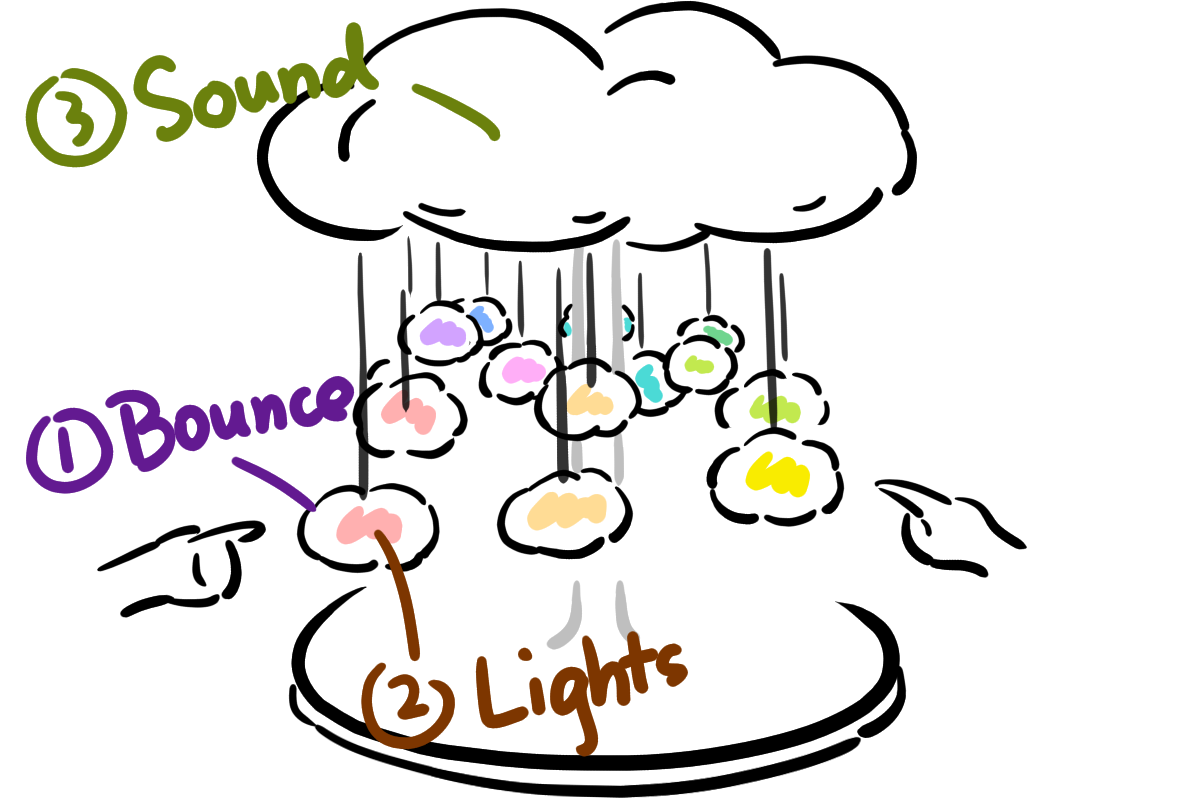
\includegraphics[width=0.5\textwidth]{Response.png}
  \caption{The multimodal response: tactile, visual, and sonic.}
  \label{fig:Response}
\end{figure}

A guided-play option, selected by holding a special cloud, allows the participant to have clouds fall into their hands in a pre-programmed sequence and play out a tune, creating a tactile and interactive musical experience.

This dual interaction scheme adapts to player expertise, creating opportunities for learning and expression for participants from varied backgrounds. Through our work, we hope to promote musical exploration and social play through an inviting appearance, an easy-to-understand mapping, and rich feedback.

Please refer to the attached animation video for an intuitive exposition of our concept.

\subsection{Background}
It has been a lasting endeavour for us to bring the joy of musical expression and performance within the reach of those without the advantage of comprehensive musical training and performances --- indeed, music, sounds, and touch are an innate expressive language shared by humankind.

However, musical ``laypeople'' tend to overcomplicate the practice of musical expression and appreciation. We have been constantly witnessing this from friends around us as well as people online: they hold back their intuitive thoughts and comments on sounds; they claim that they ``only listen for sensation's sake'' (with a negative implication) when they go to concerts; they determine that expression and creation is out of their reach because they are ignorant of musical theories; they keep reckoning their inability when they do not score well in rhythm games.

Meanwhile, we see passion surging beneath the surface. We find it a pity that many are gatekept out of this wonderful terrain that they innately connect with. We want to clear up the myth of music's meritocracy as an art form, and invite many more to the play.

Ceaseless sounds from a toy tuned-pipe metallophone in a children's corner struck us awake: what about a toy, an outlet for sound-making as well as an inlet for learning, that guides the player to connect with the music they touch? We put ourselves into the shoes of grown-up children and crafted what we believe we would enjoy --- singing, blinking, playful clouds. We hope they will find resonances around the world, so we bring them to the lovely people at NIME.

On a side note, we also hope they will remotely resonate with the machinery at Utrecht's Museum Speelklok. Who says self-playing bells must be hard metal clockwork? The flying clouds can find friends anywhere.

\subsection{Design}
\CuHum{} takes the form of a group of small clouds hanging down from a larger cloud above, which is held by a central pillar that supports the weight of other components. The clouds are made of down cotton reinforced with glue and each enfolds a tri-colour LED that gives off breathing lights. Plank makes up the the pillar and the casing of the electronic components hidden in the large cloud. Figure~\ref{fig:Sketches} provides a sketch of the overall appearance.

All interaction happens through the participant's hands or arms approaching and touching the clouds. Most of the time, touching one of the cloud triggers a multimodal response consisting of the sound of a musical note, the visuals of a changing light, and the haptics of the cloud's bouncing motion. This resembles a conventional digital musical instrument (DMI) experience.

The musical notes follow the diatonic major scale, spanning a register of two octaves, arranged along a spiral path. A revolution corresponds to an octave such that notes with the same solf\`{e}ge (full octaves apart) are aligned.

\begin{figure}[h!]
  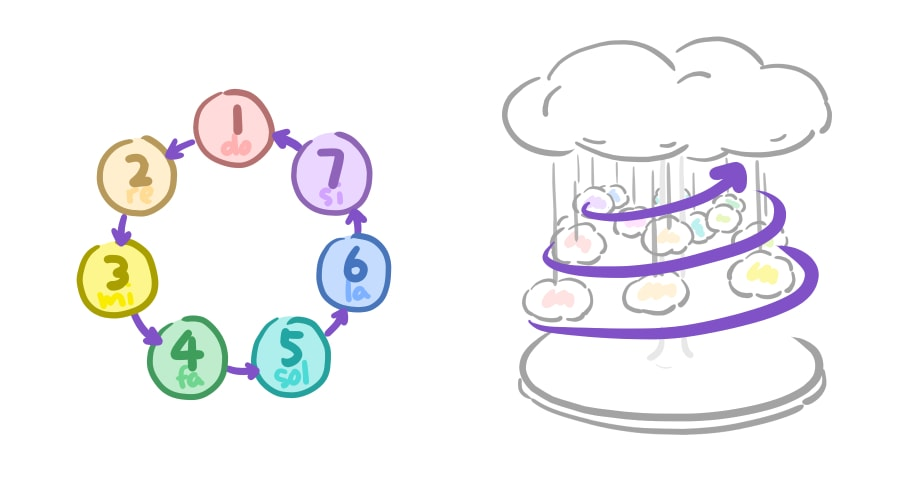
\includegraphics[width=0.75\textwidth]{../../images/CuHum_Solfege.jpg}
  \caption{The solf\`{e}ges and the spiralling alignment of the clouds.}
  \label{fig:Solfege}
\end{figure}

A specialty of \CuHum{} is its ``guided play'' mode, which is entered by the participant holding a special cloud marked by a distinctively coloured light. In this mode, clouds descend according to a pre-programmed sequence, and the participant is expected to stretch their hands or arms below all the clouds so that they fall down onto the participant's body, triggering the corresponding response, before rising back to its original position. Through this process, the participant is able to understand which notes make up the tune, as well as the timing of the music. They are also free to slightly manipulate the timings by moving their hands or arms.

In this way, we aim to realise the foremost of our intentions --- to expand the reach of the enjoyment of musical engagement. Untrained participants who pass by can try their hands on the instrument as well as go through a tangible, interactive, and understandable journey of the guided play, picking up abundant opportunities for musical exploration and learning. Of course, we expect experienced music practitioners to be getting creative with this new interface, adding to the repertoire of public performances or production techniques, or even tailoring the sounds and hardware to their imagination. We hope that \CuHum{} will be welcoming and inspiring to many.

\subsection{Implementation}
The installation can be built at variable sizes (from tabletop to human-scale) and adapts to different spaces --- we hence omit specific dimensions and give the feasible ranges in Section~\ref{sect:Perf_Notes}. A full prototype is under construction; we have cleared technical difficulties through a series of smaller unit assemblies. In this section, we provide a detailed description of the noteworthy aspects.

\subsubsection{Physical configuration}
At the top of the installation is a circuit board and a speaker, contained in a plank casing hidden in a large blob of cotton cloud. Power is supplied into the device through the central pillar. Clouds hang down from openings on the bottom of the casing. The previously-shown Figure~\ref{fig:Sketches} displays this overall configuration. Hot glue is used extensively throughout the structures.

Each cloud is driven by a brushless DC (BLDC) motor also hidden in the casing. A spindle is attached to the motor and a bundle of wires is wound around it. The wires are connected to the cloud so that it can be elevated and lowered through rotations of the motor.

\begin{figure}[h!]
  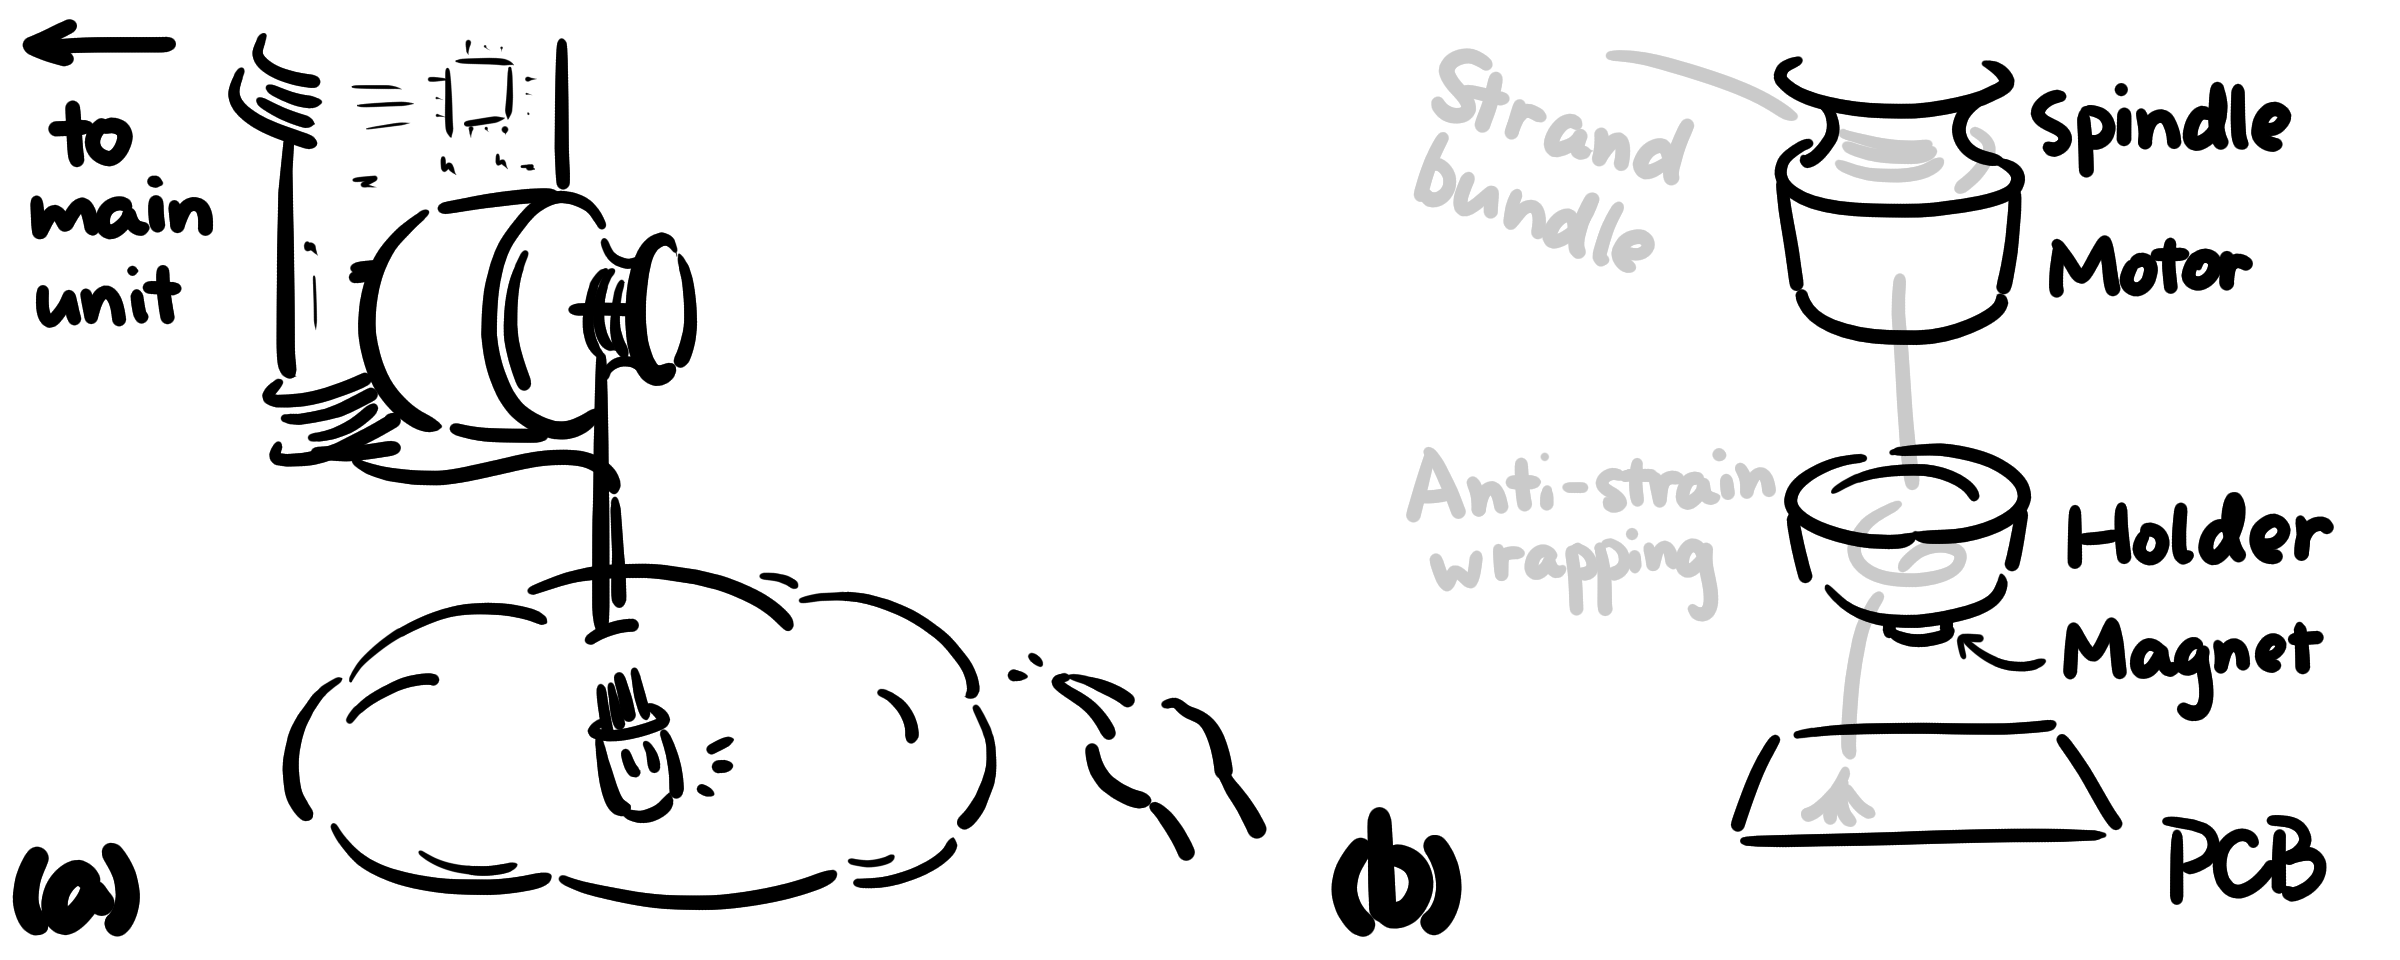
\includegraphics[width=0.75\textwidth]{Sub_Unit.png}
  \caption{Illustrations of \textbf{(a)} the composition of a sub-unit; \textbf{(b)} an exploded-view exposing how the wire bundle is wrapped.}
  \label{fig:Sub_Unit}
\end{figure}

The clouds each contains a silver-plated sewing thread, wrapped around the cotton, that serves as the electrode of capacitive sensing. This thread is fixed to an extended electrical wire by copper tape and glue. In addition, the LEDs buried in the clouds also call for electrical connections to the on-board circuitry. We hence add electrical wires to the wrapped wire bundle (totalling 5 strands of 32 AWG, strengthened with fishing wire). Figure~\ref{fig:Sub_Unit} provides a depiction of this structure.

\subsubsection{Electronics}
We design and assemble customised printed circuit boards (PCBs) for all the electronics. The entire device comprises a main unit and 16 sub-units. The main unit is responsible for delivering power and control messages to the sub-units, which each takes care of a motor and thus a cloud. Figure~\ref{fig:Block} shows a block diagram of the major components involved.

\begin{figure}[h!]
  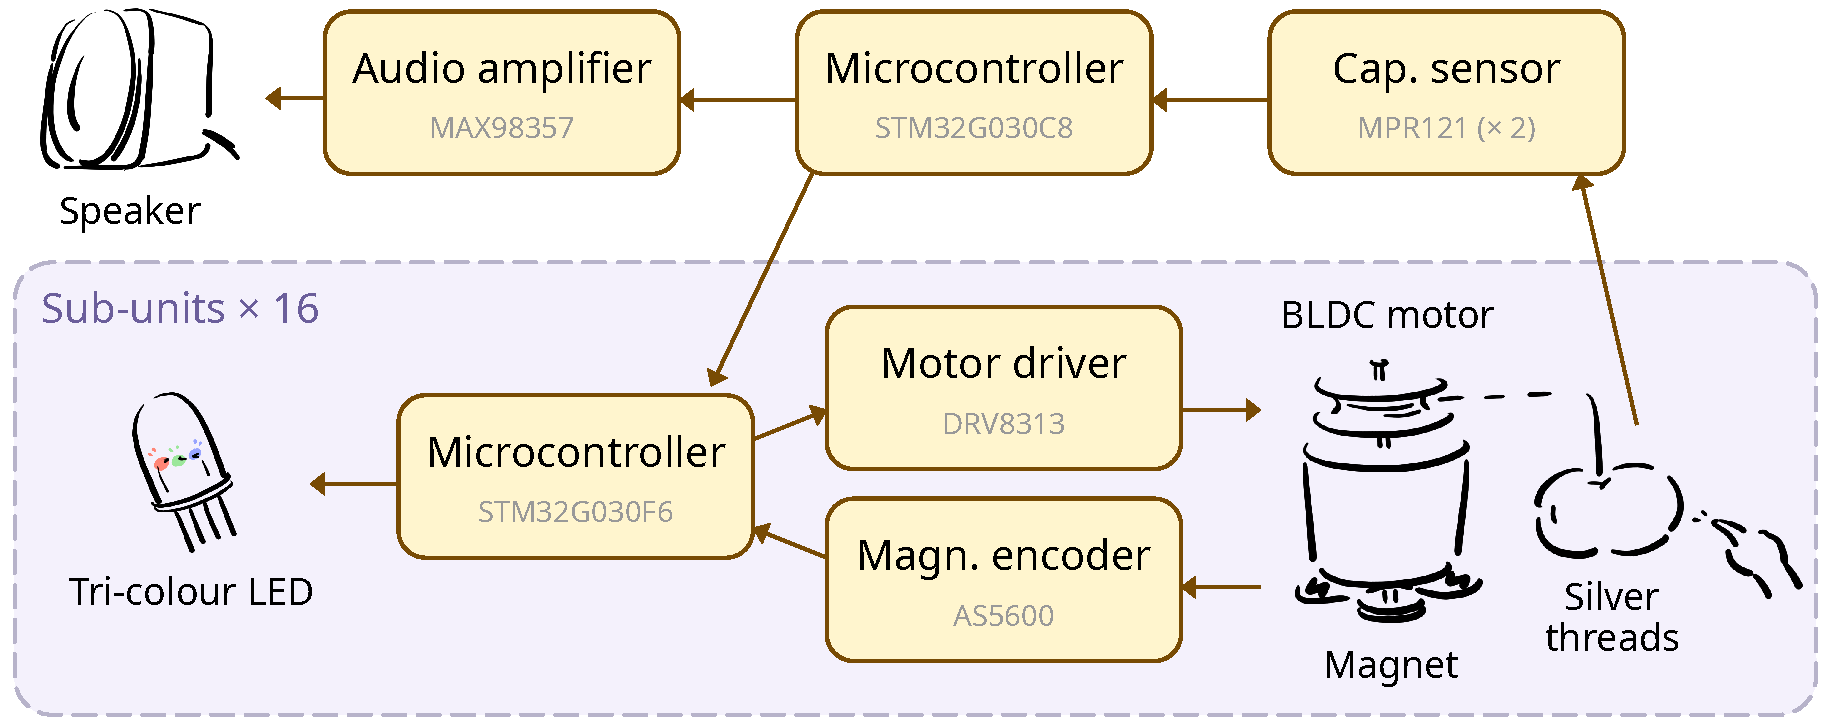
\includegraphics[width=1\textwidth]{Block.pdf}
  \caption{Block diagram of electronic components.}
  \label{fig:Block}
\end{figure}

A sub-unit contains a microcontroller communicating with a motor driver and a magnetic encoder which, complemented by the motor equipped with a magnet, forms a vector control closed loop that ensures smooth and silent movements. The main unit monitors readings of the capacitive sensor. When it determines an approaching or a touch has taken place, it sends messages to the sub-units through the SPI protocol indicating desired motor movements and LED lighting patterns. The sub-units continuously runs the motor and the LED on its own, without intervention from the main unit.

We have built multiple sub-unit assemblies (photos of which are displayed in Figure~\ref{fig:Sub-unit}) and a working main unit. As of the submission of this manuscript, a full assembly is in progress as we work through the construction of the physical structure.

\begin{figure}[h!]
  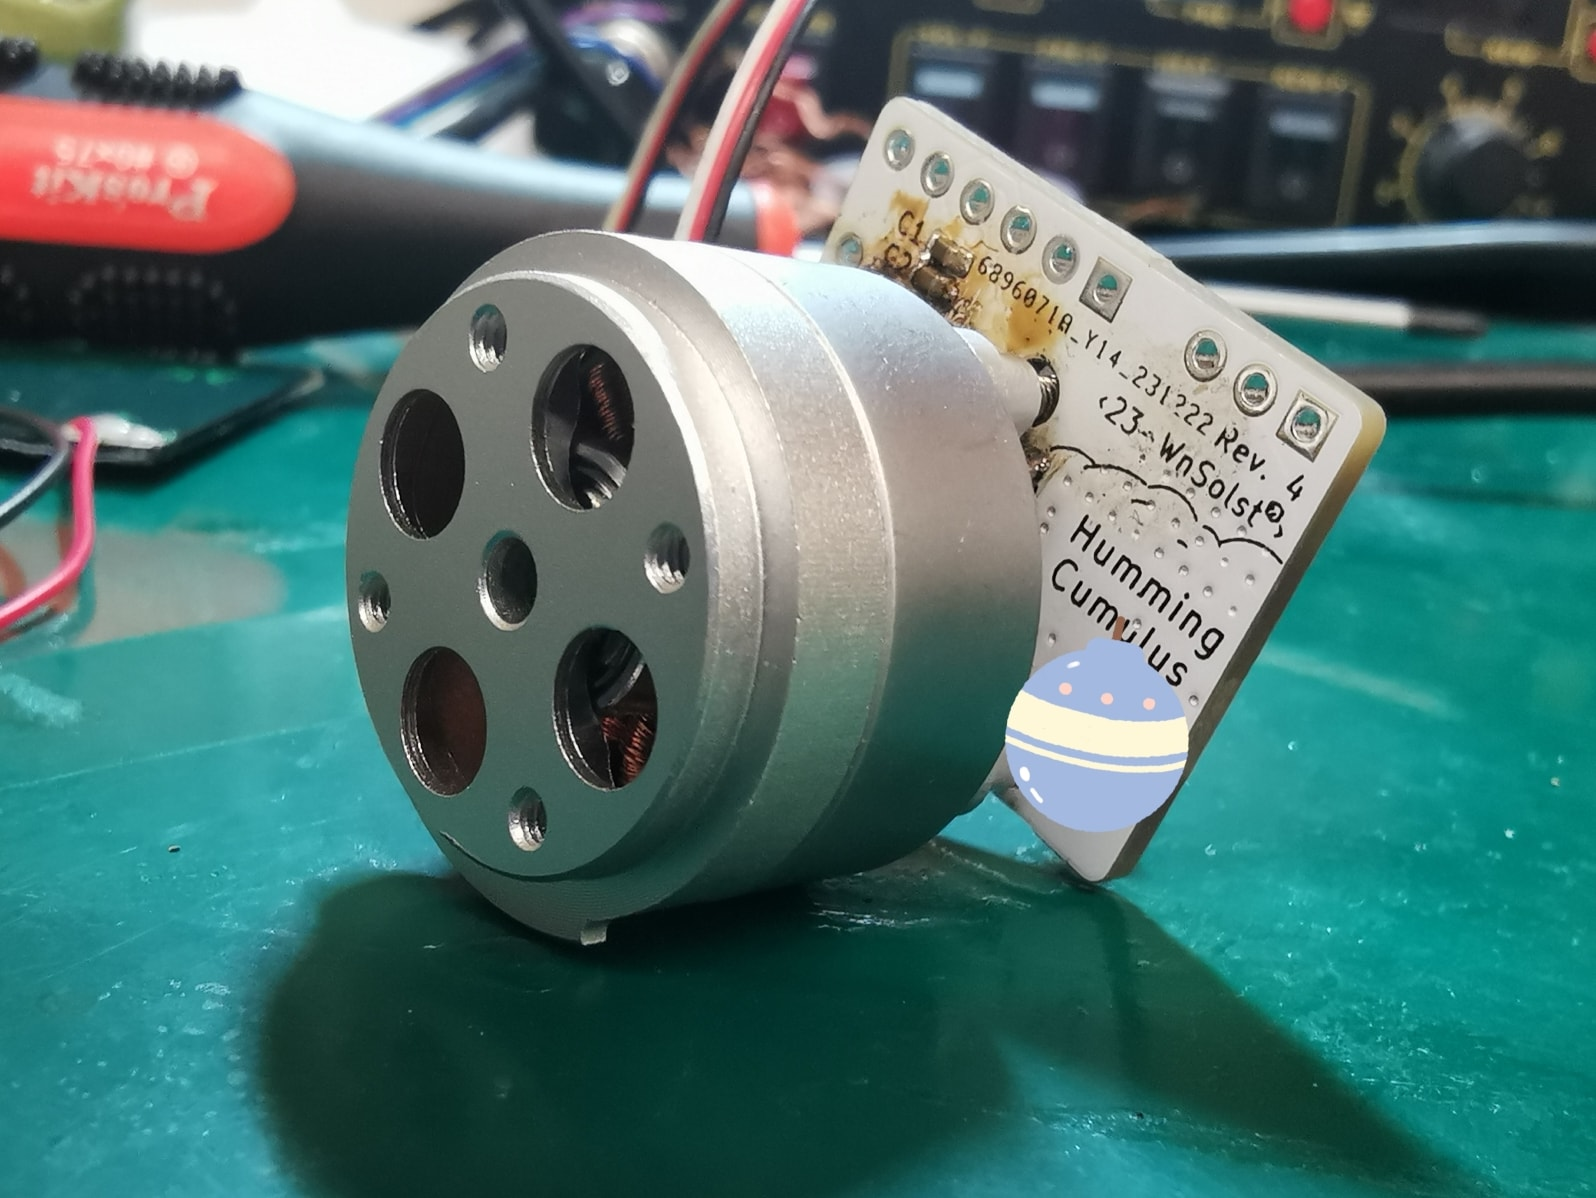
\includegraphics[width=0.42\textwidth]{Motor.jpg}
  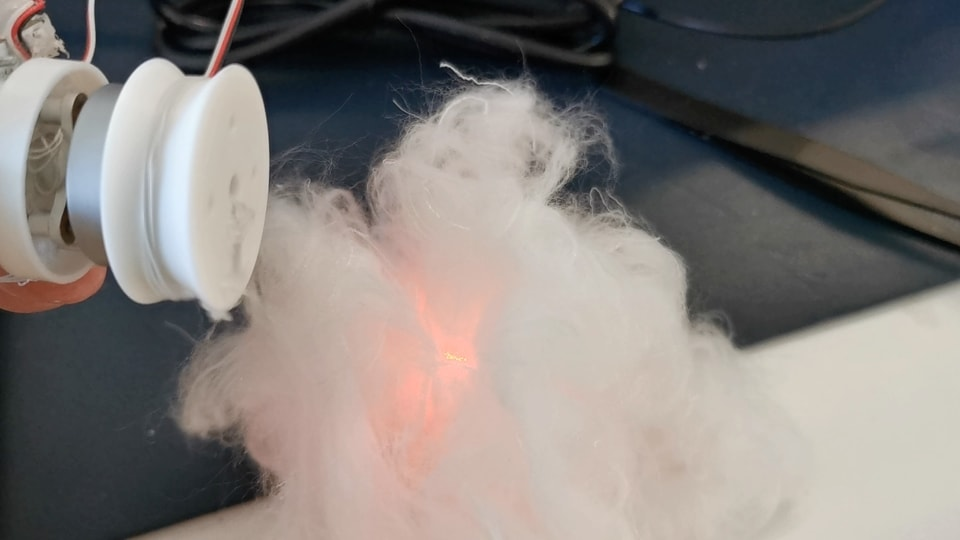
\includegraphics[width=0.56\textwidth]{Cloud.jpg}
  \caption{Photos of a sub-unit during and after assembly.}
  \label{fig:Sub-unit}
\end{figure}

We publish all design resources, including mechanical models, circuit boards, and firmware source code, at (anonymised link) under the CC BY-SA 4.0 International licence, in the hope that our implementation details will be useful to interested viewers and future designers.

\section{Performance Notes}
\label{sect:Perf_Notes}

\subsubsection{Space}
We will be able to build the installation at a variable size depending on the space available. The minimum size is $25\ \text{cm} \times 25\ \text{cm} \times 40\ \text{cm}$ (tabletop), and the maximum is $100\ \text{cm} \times 100\ \text{cm} \times 200\ \text{cm}$ (human-scale). For a tabletop realisation, we would like the table to be surrounded by at least two sides of free space (i.e., not facing a wall). For a human-scale realisation, we would like to ensure a clear space of around $2\ \text{m} \times 2\ \text{m}$. Dimensions in-between are also possible if desired. Figure~\ref{fig:Dimensions} illustrates the installation of different scales being operated. The size can be determined according to the needs and arrangements of the organisers.

\begin{figure}[h!]
  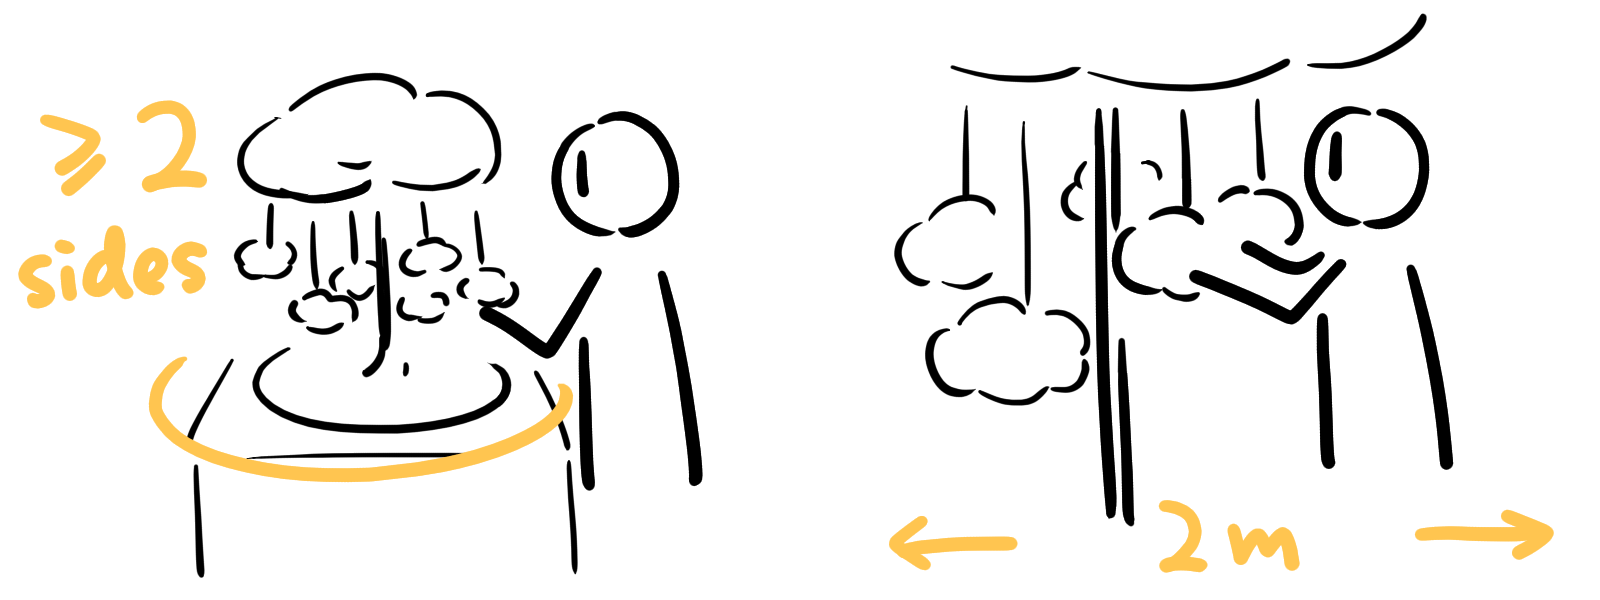
\includegraphics[width=0.8\textwidth]{Dimensions.png}
  \caption{Realisations at different scales.}
  \label{fig:Dimensions}
\end{figure}

\subsubsection{Environment}
The installation emits light, but ambient lighting conditions do not impact the effect. It works in both outdoor and indoor environments.

However, as sound and social play are crucial parts of the experience, we prefer casual environments that accept the emergence of sounds but are not noisy in their own. Hence we prefer the following from the list of provided locations:
\begin{itemize}
  \item Corridors and open spaces of the main performance venue;
  \item The HKU building `Ina Boudier-Bakkerlaan';
  \item The Nijverheid art community.
\end{itemize}

\subsubsection{Logistical}
We expect to assemble and test all circuitry beforehand, reducing on-site work to the setup of the standing structure. We thus expect set-up time to be around half a day.

\CuHum{} requires no external communication and works with a single DC power supply between 9 V and 25 V. Average power consumption is within 20 W. A mains electricity socket shall be sufficient.

\subsubsection{Feasibility}
Currently, we have built functional smaller units and will be working on a fully assembled installation at tabletop scale in the following month. We are confident that we will be accomplishing our work in time.

The authors have experience with exhibition installations and has been involved in on-site setup and troubleshooting multiple times. Members have completed similar projects (capacitive sensors, motors, sound-emitting devices) that was successfully deployed and ran without major problems. Such projects were also open-sourced and publicised.

We will take precautions to avoid material shortage in case damage happen during transport or assembly; see the following.

\subsubsection{Equipment}
We have no requirement for equipment. We will bring a pair of scissors, a pair of tweezers, screwdrivers, a piler, a hot glue gun, and a soldering iron along with corresponding material. We will also bring redundant electronic components. In case we need to repair damaged devices, necessary material can be obtained locally.

Nevertheless, we will be glad to have a AC/DC adapter rated above 20 W. The output can be either exposed wires or a DC connector. A pointer to local shops would be equally helpful.

\begin{acks}
We thank the anonymous reviewers for their effort in providing feedback.

Anonymised otherwise.
\end{acks}

% \bibliographystyle{nime-music-references.bst}
% \bibliography{nime-references.bib}

\end{document}
\endinput
